\documentclass[a4paper,10pt]{scrartcl}
\usepackage[utf8]{inputenc}
\usepackage[T1]{fontenc}
\usepackage{booktabs}
\usepackage{xspace}
\usepackage{enumitem}
\usepackage{cite}
\usepackage{graphicx}
\usepackage{tikz}
\usetikzlibrary{arrows}
\usetikzlibrary{fit}
\usetikzlibrary{calc}
\usepackage{float}
\usepackage{amssymb}
\usepackage{listings}
\usepackage[section]{placeins} % don't move figures beyond the next section heading

% this is needed for forms and links within the text
\usepackage{hyperref}

% Variables
\newcommand{\authorName}{
   Mohammed~Abu~Jayyab,
   Niklas~Baumstark,
   Tobias~Gräf,
   Amrei~Loose,
   Christoph~Michel,
}
\newcommand{\authorNameEmph}{
   Mohammed~Abu~Jayyab,
   Niklas~Baumstark,
   \textbf{Tobias~Gräf},
   Christoph~Michel,
   Amrei~Loose,
}

\newcommand{\dateFirstVersion}{\today}
\newcommand{\customer}{Karlsruhe Institute of Technology}
\newcommand{\contractor}{A company}
\newcommand{\projectName}{Broadcast Encryption\xspace}

\newcommand{\doctitle}{\projectName (Design document)}
\title{\doctitle}
\author{\authorName}
\date{\today}

% less margin
\usepackage[margin=2.5cm]{geometry}

% horizontal line
\newcommand{\HRule}{\rule{\linewidth}{0.5mm}}

% more beautiful lists
\setlist{noitemsep}
\renewcommand{\labelitemi}{$\bullet$}
\renewcommand{\labelitemii}{$\diamond$}

% create a shorter version for tables
\newcommand\addrow[2]{#1 &#2\\ }
\newcommand\addheading[2]{\textbf{\sffamily #1} &\textbf{\sffamily #2}\\ \hline}
\newcommand\tabularhead{\begin{tabular}{lp{13cm}}
\hline
}

\newcommand\addmulrow[2]{ \begin{minipage}[t][][t]{2.5cm}#1\end{minipage}%
   &\begin{minipage}[t][][t]{8cm}
    \begin{enumerate} #2   \end{enumerate}
    \end{minipage}\\ }

\newenvironment{usecase}{\tabularhead}
{\hline\end{tabular}}

% a cross
\newcommand\X{$\times$}

% templates and default styles for figures and graphics
\tikzset{>=triangle 45}
\tikzset{font=\sffamily}

\newcommand{\tmpCaption}{}
\newenvironment{illustration}[1]
{
   \renewcommand{\tmpCaption}{#1}
   \begin{figure}[h!]
   \centering
}
{
   \caption{\tmpCaption}
   \end{figure}
}


\begin{document}

\maketitle
  \begin{tabular}[t]{ll}
	Projekt:       & \quad \projektName \\[1.2ex]
	Auftraggeber:  & \quad \auftraggeber\\[1.2ex]
	Auftragnehmer: & \quad \auftragnehmer\\[1.2ex]
  \end{tabular}

\begin{tabular}{|p{3 cm}|p{3 cm}|p{5 cm}|}
\hline
\textbf{Version} & \textbf{Datum} & \textbf{Autor(en)} \\
\hline
\hline
1.0 & 29.04.2012 & \authorName \\
\hline
\end{tabular}

\tableofcontents
\clearpage

\section{Introduction}
The software CryptoCast will provide a service for sending crypted data from a server to certain
amount of people.  This will be implemented as an unidirectional connection that makes it possible for the server
to send data without knowing how many people are receiving it and without the amount of traffic caused
by a bidirectional connection.  Also the type of the sent data will not be determined by the software. So it can be
used for all sorts of data exchange. For demonstration purposes we will implement a simple audio or video stream.

The server will be able to register new users and revoke specific persons if they are not allowed to receive the cast anymore. 
The client is an app on an Android smart phone that is used for receiving, decoding and displaying the data. 
The transport between them will be implemented with TCP but that can be replaced by another transport protocoll.

The implemented encryption algorithm will be the the one by Moni Naor and Benny Pinkas, but later every other fitting the
interface can be used. This is important because there might be another more effective algorithm 


\section{Structure}
\subsection{Architecture}

\section{Package descriptions}
\subsection{Client}
The client uses a FileChooser, which can be used to select a file from the SD card of your android gadget.
As a private key is necessary to encrypt data received from a server the FileChooser is used to select a keyfile.
All servers and responding keyfiles are saved in the ServerHistory and therefore can be saved and reused after closing the client.
Every error is displayed by using a simple pop up window defined by the class ErrorFragment.
\subsection{Server}
\subsection{Communication}
\subsection{Crypto}


\section{API design}
\subsection{Package cryptocast.server}
\subsubsection{Class \lstinline|Command|}
This class represents a command and saves all legal commands.

\textbf{Constructors}
\begin{itemize}
\item \lstinline|Command()| \\
Creates a new Command with the given values

\end{itemize}


\subsubsection{Class \lstinline|Controller<ID>|}
Deals with user-interactions and therefore changes data in Model if necessary.
\begin{itemize}
\item \lstinline|<ID>|: 
\end{itemize}

\textbf{Constructors}
\begin{itemize}
\item \lstinline|Controller()| \\
Initializes a new controller with the given arguments.

\end{itemize}

\textbf{Methods}
\begin{itemize}
\item \lstinline|init()| \\
Initializes the server on start by loading data from a file.

\item \lstinline|keyGen()| \\
Tries to start a new group to which data can be sent by generating private keys.

\item \lstinline|addUser()| \\
Adds a new user and assigns a private key to that user.

\item \lstinline|revokeUser()| \\
Bans a user from the stream by adding it to the list of revoked users.

\item \lstinline|authorizeUser()| \\
Authorizes a user to watch the stream by removing it from the list of revoked users.

\item \lstinline|stream()| \\
Starts the data stream

\item \lstinline|showStatistics()| \\
Prints information about traffic

\item \lstinline|showUsers()| \\
Prints users and the keys assigned to them.

\item \lstinline|showInfo()| \\
Prints information about the data which is currently sent.

\end{itemize}

\subsubsection{Class \lstinline|User<ID>|}
This Class represents an User.
\begin{itemize}
\item \lstinline|<ID>|: 
\end{itemize}

\textbf{Constructors}
\begin{itemize}
\item \lstinline|User()| \\
Creates a User with the given name.

\end{itemize}

\textbf{Methods}
\begin{itemize}
\item \lstinline|getName()| \\


\item \lstinline|getIdentity()| \\


\end{itemize}

\subsubsection{Class \lstinline|Shell|}
Gets the arguments from the command line and deals with illegal input.

\textbf{Constructors}
\begin{itemize}
\item \lstinline|Shell()| \\
Creates a new Shell object with the given parameters.

\end{itemize}

\textbf{Methods}
\begin{itemize}
\item \lstinline|performCommand()| \\


\item \lstinline|help()| \\
Prints all commands this shell can perform with information about how to use them.

\end{itemize}

\subsubsection{Class \lstinline|ServerData<ID>|}
Contains the data which is changed by Controller and presented by View
\begin{itemize}
\item \lstinline|<ID>|: 
\end{itemize}

\textbf{Constructors}
\begin{itemize}
\item \lstinline|ServerData()| \\


\end{itemize}

\textbf{Methods}
\begin{itemize}
\item \lstinline|createNewUser()| \\
Creates and saves a new user by name.

\item \lstinline|getUserByName()| \\
Retrieves a user by name

\item \lstinline|getPersonalKey()| \\
Retrieves a user's personal key

\item \lstinline|getStreamDir()| \\


\item \lstinline|setStreamDir()| \\
Saves the directory from which is streamed.

\end{itemize}

\subsubsection{Class \lstinline|Main|}
The main method to start the server

\textbf{Constructors}
\begin{itemize}
\item \lstinline|Main()| \\


\end{itemize}

\textbf{Methods}
\begin{itemize}
\item \lstinline|main()| \\


\end{itemize}


\subsection{Package cryptocast.crypto.naorpinkas}
\subsubsection{Class \lstinline|NaorPinkasClient|}
A client in the Naor-Pinkas broadcast encryption scheme.

\textbf{Constructors}
\begin{itemize}
\item \lstinline|NaorPinkasClient()| \\
Initializes a Naor-Pinkas broadcast client

\end{itemize}

\textbf{Methods}
\begin{itemize}
\item \lstinline|decrypt()| \\
{@inheritDoc}

\end{itemize}

\subsubsection{Class \lstinline|NaorPinkasServer|}
A server in the Naor-Pinkas broadcast encryption scheme. This server is special in that it knows
 the entire polynomial and therefore all the private keys of its users. This makes the implementation
 of the interpolation algorithm a bit more efficient.

\textbf{Constructors}
\begin{itemize}
\item \lstinline|NaorPinkasServer()| \\


\end{itemize}

\textbf{Methods}
\begin{itemize}
\item \lstinline|encrypt()| \\
{@inheritDoc}

\item \lstinline|getIdentity()| \\
{@inheritDoc}

\item \lstinline|revoke()| \\
{@inheritDoc}

\item \lstinline|isRevoked()| \\
{@inheritDoc}

\item \lstinline|getPersonalKey()| \\
{@inheritDoc}

\end{itemize}

\subsubsection{Class \lstinline|NaorPinkasPersonalKey|}
A user's personal key in the Naor-Pinkas broadcast encryption scheme.

\textbf{Constructors}
\begin{itemize}
\item \lstinline|NaorPinkasPersonalKey()| \\


\end{itemize}

\textbf{Methods}
\begin{itemize}
\item \lstinline|getAlgorithm()| \\


\item \lstinline|getEncoded()| \\


\item \lstinline|getFormat()| \\


\end{itemize}

\subsubsection{Class \lstinline|NaorPinkasShare|}
A share in the Naor-Pinkas broadcast encryption scheme. It consists of a tuple
 $(r, I, g^{r P(I)})$. $t + 1$ distinct shares of this form are sufficient to restore the
 value $g^{r P(0)}$, where $t$ is the degree of the polynomial $P$.

\textbf{Constructors}
\begin{itemize}
\item \lstinline|NaorPinkasShare()| \\


\end{itemize}

\textbf{Methods}
\begin{itemize}
\item \lstinline|isComplete()| \\
{@inheritDoc}

\item \lstinline|pack()| \\
{@inheritDoc}

\item \lstinline|restore()| \\
{@inheritDoc}

\end{itemize}

\subsubsection{Class \lstinline|NaorPinkasIdentity|}
An identity in the Naor-Pinkas broadcast encryption scheme

\textbf{Constructors}
\begin{itemize}
\item \lstinline|NaorPinkasIdentity()| \\


\end{itemize}

\textbf{Methods}
\begin{itemize}
\item \lstinline|getId()| \\


\end{itemize}


\subsection{Package cryptocast.comm}
\subsubsection{Class \lstinline|SocketMulticastServer|}
This class implements channel-based communication via TCP.

\textbf{Constructors}
\begin{itemize}
\item \lstinline|SocketMulticastServer()| \\
Creates a multicast server which uses the given socket.

\end{itemize}

\textbf{Methods}
\begin{itemize}
\item \lstinline|send()| \\
Sends bytes via the channel.

\end{itemize}

\subsubsection{Class \lstinline|MessageInChannel|}
Wraps a byte-based InChannel and allows to use it as a message-based
 channel.

\textbf{Constructors}
\begin{itemize}
\item \lstinline|MessageInChannel()| \\
Creates a MessageInChannel which wraps the given inner channel.

\end{itemize}

\textbf{Methods}
\begin{itemize}
\item \lstinline|recvMessage()| \\
Receives a message via the channel.

\end{itemize}

\subsubsection{Class \lstinline|MessageOutChannel|}
Wraps a byte-based OutChannel and allows to use it as a message-based
 channel.

\textbf{Constructors}
\begin{itemize}
\item \lstinline|MessageOutChannel()| \\
Creates a new MessageOutChannel with the given OutChannel as inner channel.

\end{itemize}

\textbf{Methods}
\begin{itemize}
\item \lstinline|sendMessage()| \\
Sends the given message via the channel.

\end{itemize}

\subsubsection{Class \lstinline|MultiOutChannel|}
Multiplexes several OutChannels so that they can be used as a single
 destination.

\textbf{Constructors}
\begin{itemize}
\item \lstinline|MultiOutChannel()| \\


\end{itemize}

\textbf{Methods}
\begin{itemize}
\item \lstinline|addChannel()| \\
Adds the given channel to the list of receivers.

\item \lstinline|removeChannel()| \\
Removes the given channel from the list of receivers.

\item \lstinline|send()| \\


\end{itemize}

\subsubsection{Interface \lstinline|InChannel|}
None


\textbf{Methods}
\begin{itemize}
\item \lstinline|recv()| \\
Receives data.

\end{itemize}

\subsubsection{Interface \lstinline|OutChannel|}
None


\textbf{Methods}
\begin{itemize}
\item \lstinline|send()| \\
Sends the given data.

\end{itemize}


\subsection{Package cryptocast.util}
\subsubsection{Class \lstinline|CommandLineInterface|}
Common base class for command line programs.

\textbf{Constructors}
\begin{itemize}
\item \lstinline|CommandLineInterface()| \\
Initializes a new Cli instance

\end{itemize}

\textbf{Methods}
\begin{itemize}
\item \lstinline|run()| \\
Runs the application.

\item \lstinline|start()| \\
The main program logic (must be overridden by subclasses)

\item \lstinline|printf()| \\
Prints a string to the output stream

\item \lstinline|print()| \\
Prints a string to the output stream

\item \lstinline|println()| \\
Prints a string to the output stream after appending a newline

\item \lstinline|getErrorFormat()| \\


\item \lstinline|fatalError()| \\
Prints an error and exits

\item \lstinline|exit()| \\
Exits the application

\item \lstinline|usage()| \\
Prints usage information

\item \lstinline|getBasicUsage()| \\


\item \lstinline|printAdditionalUsage()| \\
Prints additional usage information (may be overridden)

\end{itemize}

\subsubsection{Class \lstinline|CommandLineInterface.Exit|}
Signals the exit of the application.

\textbf{Constructors}
\begin{itemize}
\item \lstinline|CommandLineInterface.Exit()| \\
Initializes a new Exit instance

\end{itemize}

\textbf{Methods}
\begin{itemize}
\item \lstinline|getStatus()| \\


\end{itemize}

\subsubsection{Class \lstinline|InteractiveCommandLineInterface|}
A framework class to implement interactive command-line interfaces. The class implements
 a read-parse-execute main loop and provides hooks for subclasses to implement the missing
 functionality.

\textbf{Constructors}
\begin{itemize}
\item \lstinline|InteractiveCommandLineInterface()| \\
{@inheritDoc}

\end{itemize}

\textbf{Methods}
\begin{itemize}
\item \lstinline|start()| \\
{@inheritDoc}

\item \lstinline|mainloop()| \\
Starts the interactive Prompt-Read-Evaluate main loop.

\item \lstinline|performCommand()| \\
Executes the given command with the given arguments. Must be implemented by subclasses.

\item \lstinline|error()| \\
Helper function to trigger an error withing a command's execution and break out to
 the main loop.

\item \lstinline|getPrompt()| \\


\end{itemize}

\subsubsection{Class \lstinline|InteractiveCommandLineInterface.CommandError|}
An error within one of the commands. Will be caught by the main loop

\textbf{Constructors}
\begin{itemize}
\item \lstinline|InteractiveCommandLineInterface.CommandError()| \\
Initializes the error

\end{itemize}

\textbf{Methods}
\begin{itemize}
\item \lstinline|getMessage()| \\


\end{itemize}


\subsection{Package cryptocast.client}
\subsubsection{Class \lstinline|StreamViewerActivity|}
This activity is responsible for decrypting the received data
 stream and viewing it.

\textbf{Constructors}
\begin{itemize}
\item \lstinline|StreamViewerActivity()| \\


\end{itemize}

\textbf{Methods}
\begin{itemize}
\item \lstinline|processStream()| \\
Processes the input stream of data

\end{itemize}

\subsubsection{Class \lstinline|ServerLoginActivity|}
This class represents the activity to connect to the server.
 Before connecting this activity start the {@link KeyChoiceActivity} to 
 let the user choose an encryption key file. When the client receives a 
 data stream the {@link StreamViewerActivity} is started to process the 
 stream and show its contents.

\textbf{Constructors}
\begin{itemize}
\item \lstinline|ServerLoginActivity()| \\


\end{itemize}

\textbf{Methods}
\begin{itemize}
\item \lstinline|connectToServer()| \\
Connects to server

\item \lstinline|checkValidAddress()| \\
Checks if server address is valid

\item \lstinline|chooseKeyFile()| \\
Shows activity to choose key file

\item \lstinline|showStream()| \\
Shows activity to view downloaded stream

\item \lstinline|processError()| \\
Processes any errors

\end{itemize}

\subsubsection{Class \lstinline|KeyChoiceActivity|}
This activity lets a user choose an encryption key file 
 which is then sent to the server for authentication.

\textbf{Constructors}
\begin{itemize}
\item \lstinline|KeyChoiceActivity()| \\


\end{itemize}

\textbf{Methods}
\begin{itemize}
\item \lstinline|chooseKeyFile()| \\
Chooses a key file

\end{itemize}


\subsection{Package cryptocast.crypto}
\subsubsection{Class \lstinline|Share.InsufficientInformationException|}
An exception that is thrown when a secret cannot be restored because
 of missing information.

\textbf{Constructors}
\begin{itemize}
\item \lstinline|Share.InsufficientInformationException()| \\


\end{itemize}


\subsubsection{Class \lstinline|LagrangeInterpolation<T>|}
Performs a lagrange interpolation of a polynomial
\begin{itemize}
\item \lstinline|<T>|: 
\end{itemize}

\textbf{Constructors}
\begin{itemize}
\item \lstinline|LagrangeInterpolation()| \\
Initializes the algorithm

\end{itemize}

\textbf{Methods}
\begin{itemize}
\item \lstinline|computeCoefficients()| \\


\end{itemize}

\subsubsection{Class \lstinline|IntegersModuloPrime|}
The field $Z/Zp$ of integers modulo a prime $p$

\textbf{Constructors}
\begin{itemize}
\item \lstinline|IntegersModuloPrime()| \\
Initializes the field

\end{itemize}

\textbf{Methods}
\begin{itemize}
\item \lstinline|add()| \\


\item \lstinline|multiply()| \\


\item \lstinline|negate()| \\


\item \lstinline|invert()| \\


\item \lstinline|zero()| \\


\item \lstinline|one()| \\


\item \lstinline|randomElement()| \\


\end{itemize}

\subsubsection{Class \lstinline|Polynomial<T>|}
A polynomial $P$ over a field
\begin{itemize}
\item \lstinline|<T>|: The type of the field's elements
\end{itemize}

\textbf{Constructors}
\begin{itemize}
\item \lstinline|Polynomial()| \\
Initializes a polynomial

\end{itemize}

\textbf{Methods}
\begin{itemize}
\item \lstinline|getField()| \\


\item \lstinline|evaluate()| \\
Evaluates the polynomial at a single point.

\item \lstinline|evaluateMulti()| \\
Evaluates the polynomial at multiple points in $O\left(n \cdot \log
 n\right)$

\item \lstinline|getCoefficient()| \\


\item \lstinline|createRandomPolynomial()| \\
Generates a random polynomial over the field

\end{itemize}

\subsubsection{Class \lstinline|Field<T>|}
Represents a field over values of type T
\begin{itemize}
\item \lstinline|<T>|: The values we work on
\end{itemize}

\textbf{Constructors}
\begin{itemize}
\item \lstinline|Field()| \\


\end{itemize}

\textbf{Methods}
\begin{itemize}
\item \lstinline|add()| \\
Adds two elements of the field

\item \lstinline|multiply()| \\
Multiplies two elements of the field

\item \lstinline|negate()| \\


\item \lstinline|invert()| \\


\item \lstinline|zero()| \\


\item \lstinline|one()| \\


\item \lstinline|randomElement()| \\


\item \lstinline|subtract()| \\
Subtracts two elements of the field

\item \lstinline|divide()| \\
Divides two elements of the field

\item \lstinline|pow()| \\
Raises an element of the field to an integer power

\end{itemize}

\subsubsection{Class \lstinline|BroadcastEncryptionServer<ID>|}
The server side of a broadcast encryption scheme.
\begin{itemize}
\item \lstinline|<ID>|: The type of the identities
\end{itemize}

\textbf{Constructors}
\begin{itemize}
\item \lstinline|BroadcastEncryptionServer()| \\
Initializes a broadcast encryption server.

\end{itemize}

\textbf{Methods}
\begin{itemize}
\item \lstinline|run()| \\
Run the worker that handles periodic group key broadcasts and sends
 queued data packages.

\item \lstinline|send()| \\
Send plaintext data to the channel. It will be encryted and broadcasted
 on the fly.

\item \lstinline|revoke()| \\
Revoke a user.

\end{itemize}

\subsubsection{Class \lstinline|BroadcastEncryptionClient|}
The client side of a broadcast encryption scheme.

\textbf{Constructors}
\begin{itemize}
\item \lstinline|BroadcastEncryptionClient()| \\
Initializes a broadcast encryption client.

\end{itemize}

\textbf{Methods}
\begin{itemize}
\item \lstinline|recv()| \\
Receive data from the channel. It is decrypted on the fly.

\end{itemize}

\subsubsection{Interface \lstinline|Decryptor<S>|}
A strategy to decrypt a single secret
\begin{itemize}
\item \lstinline|<S>|: the type of the secret
\end{itemize}


\textbf{Methods}
\begin{itemize}
\item \lstinline|decrypt()| \\


\end{itemize}

\subsubsection{Interface \lstinline|Share<S>|}
Represents a possibly incomplete piece of information to restore a secret value.
\begin{itemize}
\item \lstinline|<S>|: the type of secret.
\end{itemize}


\textbf{Methods}
\begin{itemize}
\item \lstinline|isComplete()| \\


\item \lstinline|restore()| \\
Restore the value represented by this share.

\item \lstinline|pack()| \\


\end{itemize}

\subsubsection{Interface \lstinline|BroadcastSchemeUserManager<ID>|}
Manages a set of user identites
\begin{itemize}
\item \lstinline|<ID>|: The type of the identities
\end{itemize}


\textbf{Methods}
\begin{itemize}
\item \lstinline|getIdentity()| \\


\item \lstinline|revoke()| \\
Revokes a user

\item \lstinline|isRevoked()| \\


\end{itemize}

\subsubsection{Interface \lstinline|Encryptor<S>|}
A strategy to encrypt a single secret
\begin{itemize}
\item \lstinline|<S>|: the type of the secret
\end{itemize}


\textbf{Methods}
\begin{itemize}
\item \lstinline|encrypt()| \\


\end{itemize}

\subsubsection{Interface \lstinline|BroadcastSchemeKeyManager<ID>|}
Manages the private keys of a set of users.
\begin{itemize}
\item \lstinline|<ID>|: The type of the user identities
\end{itemize}


\textbf{Methods}
\begin{itemize}
\item \lstinline|getPersonalKey()| \\


\end{itemize}

\subsubsection{Interface \lstinline|ShareCombinator<S, T>|}
Implements a strategy to merge multiple Shares into a single share with
 more information.
\begin{itemize}
\item \lstinline|<S>|: The type of the secret
\item \lstinline|<T>|: The type of the shares
\end{itemize}


\textbf{Methods}
\begin{itemize}
\item \lstinline|combine()| \\
Combines two shares.

\end{itemize}




\section{Sequences}

%\bibliography{../bibtex/references}{}
%\bibliographystyle{plain}

\section{GUI design}
The following images show prototypes of the graphical user interface.

\begin{illustration}{The main screen which is shown on program start. (The empty space is used for the logo later on))}
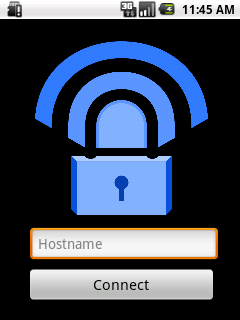
\includegraphics[width=150px]{figures/images/mainscreen.png}
\end{illustration}
\begin{illustration}{The menu which pops up after the menu button is pressed. It allows navigation between the different screens.}
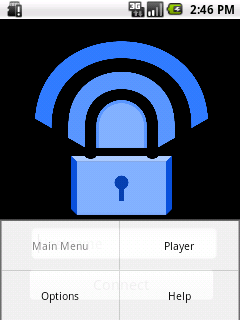
\includegraphics[width=150px]{figures/images/menu.png}
\end{illustration}
\begin{illustration}{The option screen which contains preferences, traffic data and a server history.}
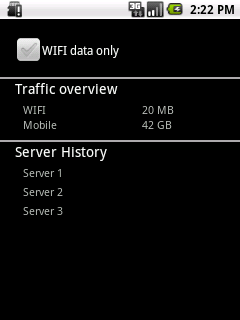
\includegraphics[width=150px]{figures/images/optionscreen.png}
\end{illustration}

\end{document}
